\documentclass[peerreview]{IEEEtran}
\usepackage{cite} % Tidies up citation numbers.
\usepackage{url} % Provides better formatting of URLs.
\usepackage[utf8]{inputenc} % Allows Turkish characters.
\usepackage{booktabs} % Allows the use of \toprule, \midrule and \bottomrule in tables for horizontal lines
\usepackage{graphicx}
\usepackage[acronym]{glossaries}
\usepackage{listings}

%\hyphenation{op-tical net-works semi-conduc-tor} % Corrects some bad hyphenation 
\makeglossaries
 
\newacronym{ppv}{PPV}{Positive Predictive Value}
 
\newacronym{npv}{NPV}{Negative Predictive Value}

\newacronym{lr}{LR}{Likelihood Ratio}

\begin{document}
%\begin{titlepage}
% paper title
% can use linebreaks \\ within to get better formatting as desired
\title{Non-Invasive Detection of Anemia (NIDA)}


% author names and affiliations

\author{Vedanshu
}
\date{8/3/17}

% make the title area
\maketitle
\tableofcontents
% \listoffigures
\listoftables
\printglossary[type=\acronymtype]
%\end{titlepage}


\IEEEpeerreviewmaketitle
\begin{abstract}
NIDA, an open-source software that noninvasively detects hemoglobin concentration using raw image from a consumer
camera and a color calibration card.The patient pull lower conjunctiva downwards with one hand while holding a color calibration
card in the other hand. Photographs are then taken and analyzed using the software. Hemoglobin measurement is a standard clinical tool
commonly used for screening anemia and assessing a patient’s response to iron supplement treatments. Anemia is a major health burden 
worldwide. Although the finding of conjunctival pallor on clinical examination is associated with anemia, inter-observer variability 
is high, and definitive diagnosis of anemia requires a blood sample. My goal was to develop a low cost and non-invasive screening test
for anemia .
\end{abstract}

\section{Introduction}

The advancement of computing technologies have revolutionized the health care facilities providing cost effective and 
remote health care platform. A number of research has been conducted for the detection of anemia using digital photographs,
however no dedicated software was developed\cite{suner2007non,10.1371/journal.pone.0153286}.
Smartphone application such as HemaApp can noninvasively monitors blood hemoglobin concentration using the smartphone’s camera and various lighting sources 
but is limited to the devices for which it has been calibrated\cite{Wang:2016:HNB:2971648.2971653}. In this paper I present 
NIDA an open-source software that can noninvasively detect hemoglobin concentration using raw image.

Anemia is considered as a proxy indicator of iron deficiency \cite{pasricha2010determinants} because it is defined as an 
abnormal iron biochemistry with or without anemia \cite{kotecha2011nutritional}. 
% Iron deficiency is caused by the poor 
% iron intake and low iron bioavailability\cite{pasricha2010determinants,bharati2015socioeconomic}. Some other factors like 
% vitamin $A$, vitamin $B_{12}$, hookworm, and malaria infection are found associated with anemia among preschool children
% \cite{pasricha2010determinants}. Iron deficiency anemia affects the physical and mental development of the human body
% \cite{pasricha2010determinants,bentley2003burden}. 
Iron deficiency reduces the learning capacity of the children aged 
below five years, decreases attentiveness, and causes low intelligence \cite{singh2014}. The consequences of anemia for 
women include increased risk of low birth weight or prematurity, perinatal and neonatal mortality, inadequate iron stores 
for the newborn, increased risk of maternal morbidity and mortality, and lowered physical activity, mental concentration, 
and productivity. Women with even mild anemia may experience fatigue and have reduced work capacity 
\cite{bentley2003burden}.Thus, anemia leads to decrease of the actual economic productivity of human resources and 
ultimately impacts on the development of the country\cite{singh2014,bentley2003burden}.

The gold standard for anemia diagnosis is ex-vivo measurement of hemoglobin concentration in whole blood. This method 
requires venepuncture and specialized equipment, which may introduce delays or be unavailable in resource-poor settings
\cite{10.1371/journal.pone.0153286}.

Hemoglobin predominantly absorbs green light and reflects red light, and as a result hemoglobin concentration affects 
tissue color\cite{setaro2002quantification}. An ``erythema index'' (EI) has been developed to objectively quantify the degree of erythema of skin 
lesions, using digital photography followed by analysis of the red and green components of images 
\cite{yamamoto2008derivation,setaro2002quantification,10.1371/journal.pone.0153286}.

\section{Problem Definition}
About 58\% children between the age 6--59 months are anemic with Hb level less than 11.0 g/dl.Non-pregnant women between age
15--49 years having Hb level less than 12 g/dl is 53.1\% and pregnant women between age 15--49 years who are anemic($<11.0$ g/dl)
is 50.3\%. Among men, anemia is less with about 23\% men being anemic with Hb level less than 13.0 g/dl\cite{nfhs-4}.

Although nutritional problem is very common in all states, it is more prevalent and severe in the particular states, whose 
performances are very poor in respect of the other important demographic and 
socioeconomic indicators. The Government of India (GOI) has named these states as Empowered Action Groups (EAG) states, 
which consist of Uttarakhand, Uttar Pradesh, Madhya Pradesh, Bihar, Odisha, Jharkhand, Chhattisgarh, and Rajasthan. The 
EAG states comprise almost 45\% of Indian population\cite{singh2014}.

There is currently no health services being provided by the government or private organizations which is cost-effective
, convenient and reaches people across all rural and urban areas. Also, no medical history is maintained of the people
which can be accessed digitally across the globe. 

\section{Proposed Solutions}
A quick and convenient delivery of health services which can reach distant areas, this will reduce footfall in  government 
hospitals, with service delivery closer-to-home. To use the best of what we have we could use the basic services already
provided to the consumer through eMitra (G2C and B2C services provided by the government of Rajasthan). Government of 
Rajasthan have set up the eMitra platform of eGovernance way back in the year 2004. Currently, covering all rural 
and urban areas in 33 districts of Rajasthan. EMitra platforms already have the access to computers, cameras and printers. 
So, a technology which could use these already available facilities to provide health services would be beneficial for the 
people. 

The solution provided in this paper aimed to detect anemia by quantifying conjunctival pallor using digital photographs 
taken with a consumer camera. Before it could be used, refinement of the image standardization technique to reduce the 
impact of device and lighting characteristics is required\cite{10.1371/journal.pone.0153286}. Following techniques 
could be used for the refinement of the image standardization.
\subsection{White calibration card}
Conjunctiva of patients are photographed in ambient lightning using a digital camera alongside an in-frame calibration
card. Mean brightness of the color calibration card's white square is used for standardization.
\subsection{Medical history and color-scale combined}
Clinical history with the use of a color-scale while assessing for conjunctival pallor. Disintermediation and robustness
are more important for this use case than confidentiality and performance, hence a blockchain database maybe preferred over 
regular databases.

\section{Research Methodology}
% The main difference between this section and the one in your report proposal is use of verb tense: there you suggested what you will do and here you will describe what you did. Be concise and precise when outlining how you researched your potential solutions. 
% Remember that your research should be guided by: 
% \begin{itemize}
% \item Relevance to the context of application  
% \item Your assessment criteria 
% \item Practicality 
% \end{itemize}
% So it may be worth commenting on your research methodology in light of the above (e.g., justifying a particular approach).  
% 
% In this section, only describe how you collected data, and explain what you did to test your criteria.  \emph{Do not include your findings in this section.}

There was a cross-sectional observational study of hospital inpatients and outpatients attending Wellington Blood and 
Cancer Centre, a regional haemato-oncology service \cite{10.1371/journal.pone.0153286}. De-identified participant data are 
available from the Dataverse which contains hemoglobin results, erythema index values, reproducibility data, and clinician
consistency values\cite{L4MDKC_2015}. Proposed solution A (``White calibration card'')\cite{anggraeni2017non,10.1371/journal.pone.0153286} 
is used as case study in the following analysis and result is compared with prior studies done using proposed solution B 
\cite{chowdhury2002taking}. Photographs of the case study were taken at a distance of approximately 40 cm, and framed to 
include the eye and color calibration card within the same image and the same coronal plane. Automatic focus was used
throughout. Photographs were taken without flash and saved using the RW2 file format . The internal white balancing 
feature was utilized, using a white sheet of paper as a reference.

Images were loaded in OpenCV and were standardized using a previously established method\cite{zhao2013quantitative}.
Each images was split into its 8-bit red, green and blue channels using the OpenCV $cv::split()$ function. From the image 
white square was selected and its mean brightness was calculated. Each channel's brightness was adjusted by multiplying 
its brightness by $200/M_B$, where $M_B$ is the mean brightness of the color calibration card's white square. Then each 
channels were merged to produce 24-bit white-balanced image and saved for future assessment. The other set of the 
standardized color channels was then used for EI analysis.

The EI was determined using the equation reported by Yamamoto et al\cite{yamamoto2008derivation,bersha2010spectral}.
\begin{equation}
 EI = \log{S_{red}} - \log{S_{green}}
\end{equation}
where, $S$ is the brightness of the conjunctiva in the relevant color channel. Since, these were 8-bit color channels, 
the $\log$ value has to be scaled for results within the pixel scale of 0--255. The scaling $\log$ function used was:
\begin{equation}
 f(p) = 255 * \log{p}/\log{255}
\end{equation}
The function was applied to all three color channels. Following this the log green channel was subtracted from the log red channel
using the OpenCV $cv::subtract()$ function. Palpebral portions of the conjunctiva was selected individually using a polygon tool
made in QML and OpenCV. The intensity of the pixel brightness of the selection is the EI.
In the appendix code used for this process is provided.

\section{Analysis and Interpretation}

Digital EI analysis using the data\cite{L4MDKC_2015} showed that it identified 70\% of images as anemic or not anemic whereas 
clinician assessment showed that clinicians were less accurate with images, scoring mean 60.33\%. Digital EI analysis resulted
in a higher positive likelihood ratio and stronger statistical association between conjunctival pallor and proven anemia than
assessment by clinicians. Table \ref{tab:ei} shows test characteristics of conjunctival pallor assessment by three clinicians compared with digital EI analysis
for detection of anemia (hemoglobin $< 11.0$ g/dl). Threshold of $< 18.14$ for anemia detection used for conjunctival
EI values from photographs\cite{10.1371/journal.pone.0153286}.

\begin{table}
\centering
\begin{tabular}{l c c c c}
\toprule 
 & Digital Image EI & Clinician 1 & Clinician 2 & Clinician 3 \\ 
\midrule 
\acrshort{ppv} & 0.76 & 0.59 & 0.62 & 0.71 \\ 
\acrshort{npv} & 0.67 & 0.63 & 0.52 & 0.58 \\ 
Positive \acrshort{lr} & 3.39 & 1.16 & 1.29 & 2.02 \\
Sensitivity & 0.57 & 0.88 & 0.62 & 0.58 \\ 
Specificity & 0.83 & 0.24 & 0.52 & 0.71 \\
\bottomrule
\end{tabular}
\smallskip 
\caption{ Comparison of palpebral conjunctival EI with clinician assessment}
\label{tab:ei}
\end{table}

Prior studies shows that solution B have improved test characteristics by combining a clinical history with the use of a color-scale while 
assessing for conjunctival pallor, increasing sensitivity from 74\% for pallor alone to 83\% when medical history 
and color-scale were combined. However sensitivity remained low for milder degrees of anemia \cite{chowdhury2002taking}.
Sensitivities (Hb $< 11$ g/dl)and specificities (Hb $>11$ g/dl) improved consistently over the three sequential phases of clinical assessment based 
on pallor, medical history and the color scale in each category of anemia as seen in Table \ref{tab:imp_ei}. 

\begin{table}
\centering
\begin{tabular}{l c c c}
\toprule 
 & (I) & (II) & (III) \\
 & Clinical pallor & I + Medical history & II + Color scale \\ 
\midrule 
Sensitivity & 0.74 & 0.78 & 0.83 \\ 
Specificity & 0.76 & 0.85 & 0.91 \\
\bottomrule
\end{tabular}
\smallskip 
\caption{Sensitivity, specificity for detecting anemia at three sequential phases of assessment}
\label{tab:imp_ei}
\end{table}

Although the method of image standardization used by solution A is cost effective and less complex it was not able 
to eliminate the effect of ambient lightning on EI. Using the color scale in assessing conjunctival pallor improved 
both sensitivity and specificity although an important point to note is that in each subsequence phase of clinical
assessment relatively, greater improvement occurred in specificity than in sensitivity. Perhaps the evidence indicates
the improved ability to correctly diagnose non-anemic subjects who were inaccurately diagnosed in the preceding solution.
 In real situations the accuracy of clinical assessment by the paramedics may decrease over time, especially in the absence 
 of regular examination of patients; thus, occasional training may be necessary to maintain their level of skills.
On the other hand, implementation of solution B would require larger database and online access to it, which would increase 
its complexity. A blockchain database would be preferable here so that the transactions would be shared
on a peer-to-peer basis across the densely connected nodes across different locations. End users generating the transactions 
connect to (say) 5 of these nodes, so it doesn’t matter if a few communication links go down. And if one or two nodes fail 
completely on any given day, nobody feels a thing, because there are still more than enough copies to go round. As it 
happens, this would combine low cost systems and high redundancy. 

\begin{figure}[htp]
 \centering
 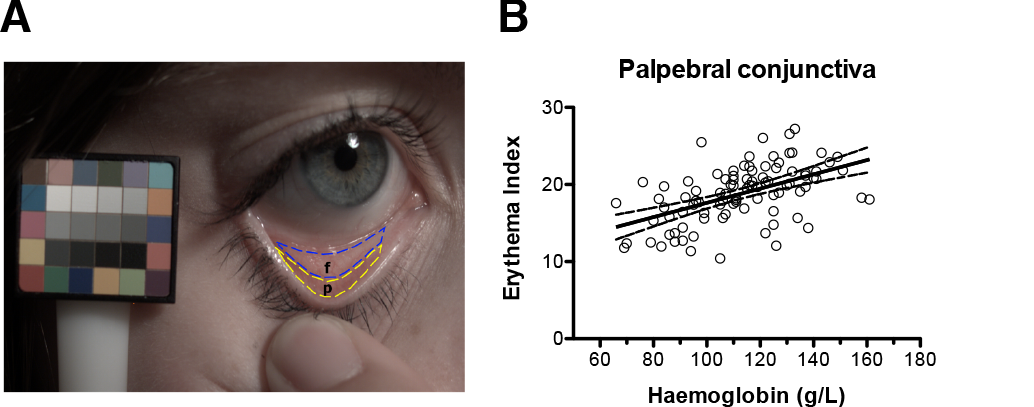
\includegraphics[width=\linewidth]{img.png}
 \caption{Relationship between erythema index and hemoglobin for palpebral}
 \label{fig:0}
\end{figure}


Fig.\ref{fig:0} (A) Representative calibrated image from a non-anaemic participant showing the palpebral (p) of the conjunctiva. 
The in-frame color calibration target is shown. (B) Relationship between palpebral conjunctival EI derived from images and 
measured hemoglobin. Solid line represents best fit by linear regression.
\section{Usage}
\subsection{Data input}
Before any analysis can be done, an input image file that focuses conjunctiva and a color calibration card must be read, processed and 
loaded in NIDA. For this click on $ File->Open$ and select the image. The image will be loaded in the window as follows
\begin{figure}[htp]
 \centering
 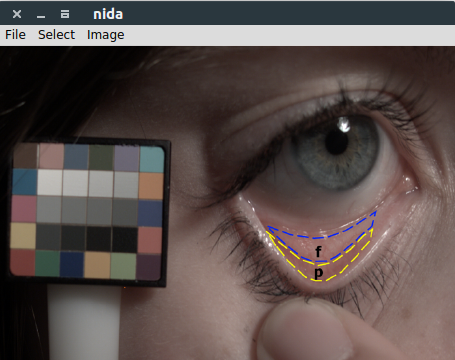
\includegraphics[width=0.5\linewidth]{main.png}
 \caption{Main window with image loaded}
 \label{fig:1}
\end{figure}

\subsection{Standardization technique}
Before the image could be used,refinement of the image to reduce the impact of device and lighting characteristics is required.
Click $Select->Rectangle$ and select the white square in the calibration card.
\begin{figure}[htp]
 \centering
 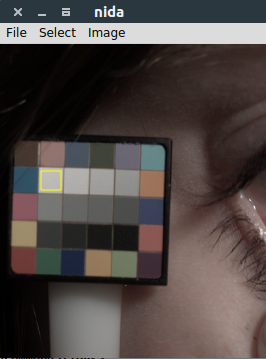
\includegraphics[width=0.5\linewidth]{rec.png}
 \caption{White square of calibration card selected}
 \label{fig:2}
\end{figure}

\subsection{Image analysis}
Since the image has been loaded successfully, it's time to do the analysis. Click $Image->Split$ and then $Image->ROI$. 
The image with be loaded in $OpenCV$; standardization algorithms will be performed.

\subsection{Getting the EI}
Palpebral portions of the conjunctiva will be selected using the `polygon' tool to maximise sampling area and measured on the EI image.
Click $Select->Polygon$ and select the conjunctiva, the yellow portion in the image shown below is the palpebral conjunctiva. Click 
$Image->Palpebral$ and a dialog box will be opened giving the EI.
\begin{figure}[htp]
 \centering
 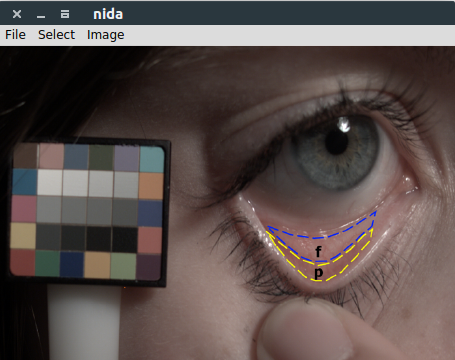
\includegraphics[width=0.5\linewidth]{main.png}
 \caption{Yellow portion of the image is conjunctiva}
 \label{fig:3}
\end{figure} 

\section{Conclusions and Recommendations}
NIDA is an open-source software that noninvasively monitors the hemoglobin concentration using digital photographs.
In this study two image standardization technique was analyzed and reported method of quantifying erythema of skin 
lesions (the erythema index, EI) to quantify conjunctival pallor from digital images. White calibration card image 
standardization technique proved to be the most cost effective of the alternatives. Medical history and color-scale combined 
image standardization technique, though a viable option in other contexts, was shown to lack adaptability.

Non-invasive screening for anemia could have numerous applications, particularly in resource-poor settings. A 
dedicated open-source software to automate image analysis and to predict risk of severe anemia was developed. 
This study suggest that NIDA has potentials for noninvasive detection of anemia and provide a means of health 
services to wider audience particularly poor districts in India especially EAG states. To validate 
the results, a larger national and international study that includes more demographic will need to be deployed.
% Conclusion shows what knowledge comes out of the report. As you draw a conclusion, you need to explain it in terms of the preceding discussion. You are expected to repeat the most important ideas you have presented, without copying. Adding a table/chart summarizing the results of your findings might be helpful for the reader to clearly see the most optimum solution(s). 
% 
% It is likely that you will briefly describe the comparative effectiveness and suitability of your proposed solutions. Your description will logically recycle language used in your assessing criteria (section \ref{sec:criteria}): ``Solution A proved to be the most cost effective of the alternatives'' or ``Solution B, though a viable option in other contexts, was shown to lack adaptability''.  Do not have detailed analysis or lengthy discussions in this section, as this should have been completed in section X. 
%  
% As for recommendations, you need to explain what actions the report calls for. These recommendations should be honest, logical and practical. You may suggest that one, a combination, all or none of your proposed solutions should be implemented in order to address your specific problem. You could also urge others to research the issue further, propose a plan of action or simply admit that the problem is either insoluble or has a low priority in its present state.   
% 
% The recommendations should be clearly connected to the results of the report, and they should be explicitly presented. Your audience should not have to guess at what you intend to say.  

% \appendices
% \section{What Goes in the Appendices} \label{App:WhatGoes}
% The appendix is for material that readers only need to know if they are studying the report in depth. Relevant charts, big tables of data, large maps, graphs, etc. that were part of the research, but would distract the flow of the report should be given in the Appendices. 
% \section{Formatting the Appendices} \label{App:Formatting}
% Each appendix needs to be given a letter (A, B, C, etc.) and a title. \LaTeX will do the lettering automatically.


\bibliographystyle{IEEEtran}
\bibliography{references}
\end{document}


